%Introduction

\chapter{Introduction}
\label{sec:introduction}

%\chapter{Nucleation}
%\label{sec:nucleation}
%
\section{Nanotechnology}
\label{sec:nanotechnology}

Not many scientists can claim to have envisioned an entirely new field of
physics, but it is not an overstatement to say that the field of
\emph{nanotechnology} was developed in large parts due to one of the most
brilliant physicists of the 20th century, Richard Feynman. In his talk ``There's
Plenty of Room at the Bottom---An invitation to enter a new field of
physics''\autocite{Feynman_TherePlentyRoom_1960} he challenges scientists to
construct devices and compounds that only consist of a few tens or hundreds of
atoms. Such objects usually turn out to be a few nanometres ($10^{-9}$~m) in
diameter, giving rise to the field's name. It is astounding to read through the
transcript of Feynman's talk from today's perspective, as it is filled with
ideas that are very much a reality now. For example, he devises the
miniaturisation of the computer and even mentions the concept of a facial
recognition system. One of the reasons Feynman gives for his wish for this field
to be developed is cost effectiveness. Scaling everything down in size decreases
the amount of materials needed drastically. As a side effect one ends up with
much smaller and potentially more powerful devices.

Feynman noted that in order to effectively use nano-scale devices one needs to be
able investigate these small structures down to the atomic level, something that
was not possible with the electron microscopy methods available at that time.
This became a practical reality with the invention of the \ac{STM} in
1981,\autocite{Binnig_ScanningTunnelingMicroscopy_1986} which secured its
inventors the Nobel prize in 1986. Figure~\ref{fig:STM} shows an image produced
with such a microscope.
%
\begin{figure}[htb]
    \centering
    \subfloat[\label{fig:STM}]{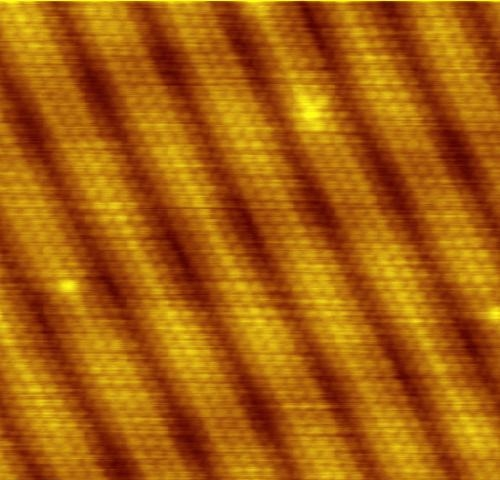
\includegraphics[width=0.35\textwidth]{other-pics/Atomic_resolution_Au100.png}}\hspace{0.05\textwidth}
    \subfloat[\label{fig:IBM}]{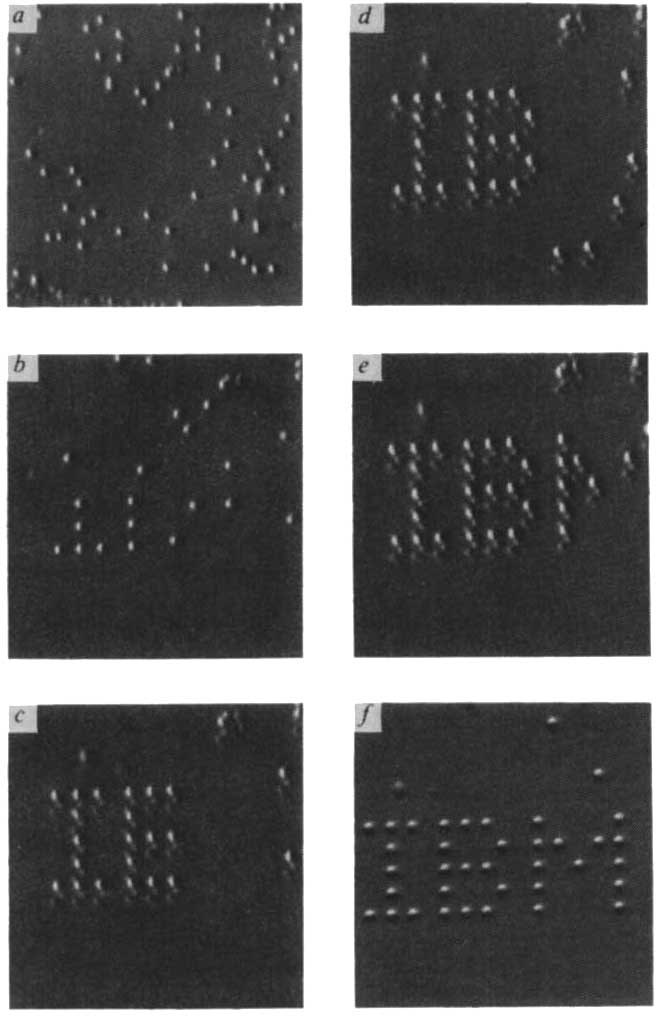
\includegraphics[width=0.35\textwidth]{other-pics/ibm.png}}
    \caption{\protect\subref{fig:STM} \acs{STM} image of a clean gold (100) surface showing atomic resolution. The ridges are a result of surface reconstructions. The image is part of the public domain. \protect\subref{fig:IBM} \acs{STM} image of Xenon atoms arranged on a nickel (110) surface in a pattern resembling the IBM logo. Reprinted by permission from Springer Nature Customer Service Centre GmbH: Springer Nature, \citetitle{Eigler_Positioningsingleatoms_1990a}\autocite{Eigler_Positioningsingleatoms_1990a}, \textcopyright 1990.}
    \label{fig:STMexamples}
\end{figure}
%
One problem with \ac{STM} imaging is that it only works on conductive surfaces.
However, this was resolved with the introduction of the \ac{AFM}, which does not
rely on a tunnelling current to produce atomic
resolution.\autocite{Binnig_AtomicForceMicroscope_1986} The technology was
perfected to such a degree that it became possible to move individual atoms and
arrange them in almost any pattern imaginable
(figure~\ref{fig:IBM}).\autocite{Eigler_Positioningsingleatoms_1990a}

In the last part of his talk, Feynman speaks about how ``atoms on a small scale
behave like nothing on a large scale, for they satisfy the laws of quantum
mechanics''. This property has found application in so-called nano-particles,
which refers to molecules or chemical compounds in general with the size of a
few nanometres. Belonging to this group are for example the
\emph{Buckminsterfullerenes} (or short fullerenes) discovered by
Kroto\autocite{Kroto_C60Buckminsterfullerene_1985} or carbon
nano-tubes\autocite{Iijima_Helicalmicrotubulesgraphitic_1991} and their
discovery helped fuelling the push for nanotechnology even further. It was
however not until the beginning of the 21st century, that nanotechnology gained
traction by securing public funding like from the National Nanotechnology
Initiative, a U.S. American federal government program. This increase in
research funding gave rise to lots of interesting scientific projects like the
``Nanocar''\autocite{Kudernac_Electricallydrivendirectional_2011} or Graphene
transistors.\autocite{Wu_Highfrequencyscaledgraphene_2011} Today, the technology
is present in many consumer products with over 800 goods reported to contain
nanotechnology.\autocite{Vance_Nanotechnologyrealworld_2015}

\section{Cluster Science}
\label{sec:ClusterScience}

A term that is often used for chemical compounds used in nanotechnolgy is
\emph{cluster}, however, the definition of the term is still debated.
Originally, it was proposed as ``an appropriate one [term] for a finite group of
metal atoms which are held together mainly, or at least to a significant extent,
by bonds directly between the metal atoms, even though some non-metal atoms may
also be intimately associated with the
cluster''.\autocite{Cotton_MetalAtomClusters_1964} However, this definition
limits itself only to the fraction of metal atoms in the periodic table and the
term is not necessarily used in this form today. The most accurate definition of
a cluster is perhaps given through size, as almost any chemical compound with a
finite number of atoms of $2$--$10^n$ ($n\lessapprox 7$) atoms is referred to as
a
cluster.\autocite{Johnston_Atomicmolecularclusters_2002,Wales_Energylandscapes_2003}
Therefore, clusters are structures, that are of intermediate size, bridging the
gap between small molecules and bulk solids,\footnote{It should be noted that
very large organic compounds like peptides are usually not considered clusters,
and are exempt from this definition.} and they appear naturally when discussing
nucleation phenomena and nano-particles. 

Clusters can be divided into several groups that are characterised by the type
of atoms comprising the cluster and therefore its electronic bonding situation.
For example, molecular clusters, which, due to their closed electronic shells,
mainly interact inter-molecularly via weak van-der-Waals forces. However, the
intra-molecular interactions are usually of covalent nature. Such clusters are
found for simple molecules, such as water,\autocite{Liu_WaterClusters_1996}
ammonia\autocite{Beu_Structureammoniaclusters_2001} or carbon
dioxide.\autocite{Takeuchi_GeometryOptimizationCarbon_2008} Moreover,
semi-conductor clusters are bound much more strongly by covalent interactions.
Their name stems from the type of atoms that make up the cluster as they are
semi-conductors in the solid state. Most famously, this group includes the
already mentioned carbon
fullerenes\autocite{Kroto_C60Buckminsterfullerene_1985}, but also other
semi-conductors like silicon\autocite{Zhu_Structuresstabilitiessmall_2003a} and
germanium.\autocite{Pacchioni_Silicongermaniumclusters_1986} If a cluster is not
monoatomic and the difference in the electronegativity of the atoms is large
enough the covalent bonding situation can change to ionic.

In this thesis, two types of clusters are more important, monoatomic metal and
rare gas clusters. The bonding situation in metal clusters is particularly
interesting, because of the high degree of delocalisation and non-directional
bonding. To describe this situation, several bonding models have been developed.
The most simple one is perhaps the \emph{liquid drop model} which approximates
the metal cluster as a uniform conducting sphere, i.e. it is a classical
electrostatic model. The liquid drop model does not give rise to an electronic
structure, which is resolved in the \textit{spherical jellium model}. In this
model the cluster is modelled as a uniform, positively charged sphere filled
with an electron gas, which is solved using the \textit{Schr\"odinger equation}.
This gives rise to quantised electron energy levels and therefore an electronic
shell structure. For metal clusters of not too many atoms it is also possible to
use accurate quantum chemical methods, which will be introduced in
chapter~\ref{sec:basicsofQC}.

Rare gas clusters can form at very low temperatures, when the average kinetic
energy of the rare gas atoms is smaller than the weak dispersive forces between
them. The reason they interact so weakly is because of their closed shell
electronic structures, allowing for neither covalent nor ionic bonding. As
dispersive interactions are a correlation effect of the electrons, it is
difficult to describe them accurately with quantum chemical methods. However,
the interaction can be approximated by simple models like, for example, the
London formula.
%
\begin{align}
    V_\text{disp}=-\frac{C_6}{r^6},\quad C_6=\frac{3\alpha^2I}{4\left(4\pi\varepsilon_0\right)^2}
\end{align}
%
Here, $I$ is the ionisation potential and $\alpha$ is the atomic polarisability.
In combination with a term describing the repulsive contribution to the energy,
the Lennard-Jones potential can be derived, which is in good agreement on
structure and energy with experimental results for rare gas clusters. The
Lennard-Jones potential will be explained in more detail in
chapter~\ref{sec:energylandscapes}.

\section{Fundamental Questions in Cluster Science}
\label{sec:FundamentalQuestionsinClusterScience}

%%%%%Topology

Another interesting question is how many stable structures exist for a given
number of $N$ atoms. For this, it is useful to define the potential energy
surface which is a function of all $3N$ atomic coordinates and maps them to
their energy with respect to the employed interaction potential. This is only
allowed if the motion of the nuclei is decoupled from the motion of the
electrons (Born-Oppenheimer approximation,
section~\ref{sec:bornoppenheimerapproximation}). In this case a stationary point
on the potential energy surface corresponds to a stable cluster structure. Thus,
it is equivalent to ask the question of how many local minima are supported by
the multi-dimensional potential energy surface. There is no analytical solution
to this and it very much depends on the type of interaction that is chosen to
describe the cluster. However, observations
suggest\autocite{Tsai_Useeigenmodemethod_1993} that the growth is exponential,
to be precise asymptotically
exponential.\autocite{Stillinger_Packingstructurestransitions_1984,Stillinger_Exponentialmultiplicityinherent_1999}

%%%%Greg-Newton

%The reason why clusters are studied so extensively lies within their broad range
%of properties due to the various different sizes. In smaller clusters,
%interesting quantum effects can be observed, which gives rise to the whole field
%of nano science. This field, which was most famously inspired by an article by
%Richard Feynman,\autocite{Feynman_TherePlentyRoom_1960} is thriving today.
%Because clusters are finite objects, they have a boundary that interfaces with
%their environment. A similar situation can be found in bulk surfaces, as the
%surface atoms (or atoms at the boundary in case of clusters) have lower
%coordination numbers than bulk atoms. This under-coordination gives rise to
%interesting chemical reactivity and in some case even catalytic activity.
%
%As the clusters grow in size, their properties become more and more bulk-like,
%because the electronic states are no longer quantised but quasi-continuous.
%Understanding these growth behaviours could help to unravel questions around
%crystal growth or at which size metallic conductivity can be first observed. 
%
%In this thesis, three projects related to cluster science, are investigated.
%First, the theoretical background required to carry out the calculations will be
%reviewed and a quick overview of the program package \textsc{Spheres} developed
%in this thesis will be given. The final three sections contain the results of
%the investigations. A special type of hollow gold clusters will be investigated
%in chapter~\ref{sec:goldendualfullerenes} with respect to their geometry and
%stability. These clusters show an interesting connection to the carbon
%fullerenes. Rare gas clusters are subject of
%chapters~\ref{sec:fromstickyhardspheretoLJtypeclusters} and
%\ref{sec:thegregorynewtonclusters}. The investigations in these chapters are
%focused on clusters interacting via interaction potentials that describe
%dispersive effects. The last chapter also uses graph theoretical methods to
%investigate the connectivity of the clusters with respect to the Icosahedron.
%Each project will be introduced more thoroughly in the beginning of the
%respective chapter.

